\pagebreak
\chapter{Entwicklung des Prototyps}

In diesem Kapitel werden alle Schritte, die in die Kreation des Spiels hineingeflossen sind, beschrieben. Die Entwicklung des Prototypen fing mit der Idee des Themes an und durchlief mehere Phasen bis zur finalen Version des Spiels. Bei jeder dieser Phasen wurden viele Optimierungen gemacht und Fehler ausgebessert. 


\section{Idee und Thema des Spiels}


\begin{description}
  \item [Einführung in die Ausgangsidee des Spiels]
    Wegen des Vorwissens über Unity, welches in der 1 \& 2.ten Klasse unterrichte wurde war die Ausgangsidee für das Spiel war eine einfache Wahl. Die fast einfachste und am weitesten verbreitete Kategorie von Spiel ist ein \gls{jumprun} \footnote[1]{Bedeutung: Spring \& Lauf. Ein Spiel in dem man mit Springen und Laufen ein Ziel erreichen muss.}. 

    \begin{quote}
      \emph{\glqq Ein Merkmal (von Jump'n'Run Spielen) sind die Plattformen. [...] Typisch beim Jump'n'Run ist das Verlieren\grqq}~\cite[1:42-1:57]{ArtOfGaming}
    \end{quote}
    
    Ein Jump'n'Run würde einerseits kreative Freiheit über das Theme geben, aber auch die Möglichkeit bieten viele Aspekte der Spielentwicklung in dieser Diplomarbeit zu präsentieren.

  \item [Beschreibung des gewählten Themas und dessen Bedeutung]
    Da das Spiel nicht an der realen Welt angelegt sein soll, kam die Überlegung eine Traumwelt zu bauen. In dieser gäbe es die Freiheit den Charakter, die Gegner und alle anderen Assets in verschiedenen Stilen zu designen. Damit wird auch für die Spieler dieses Prototypen klar das das gewählte Theme Fantasy ist. Diese Themenwahl erleichtert zudem dem Game-Designer die kreative Gestaltung.

  %\item [Erläuterung der Inspirationsquellen und kreativen Einflüsse]
  
\end{description}

\pagebreak

\section{Konzept und Anfangsschritte}
Das Konzept und die Anfangsschritte unterteilen sich in die folgenden Gebiete: 
\begin{itemize}
  \item Ideenfindung und Konzeptzeichnung für den ersten Prototypen (V1)
  \item Auswahl des Spielthemas und Design des Hauptcharakters
  \item Überlegung der grundlegenden Charaktersteuerung und Charakterfähigkeiten
\end{itemize}

Die ersten Scritte bei dem Entwickeln eines Videospiels sind beginnen immer mit einem Brain-Storming. Die ersten Ideen für diesen Prototypen waren das Theme, das Layout des ersten Levels und das ungefähre Design des Charakters.

  \begin{figure}[h]
    \centering
    \begin{minipage}[b]{0.45\textwidth}
      \centering
      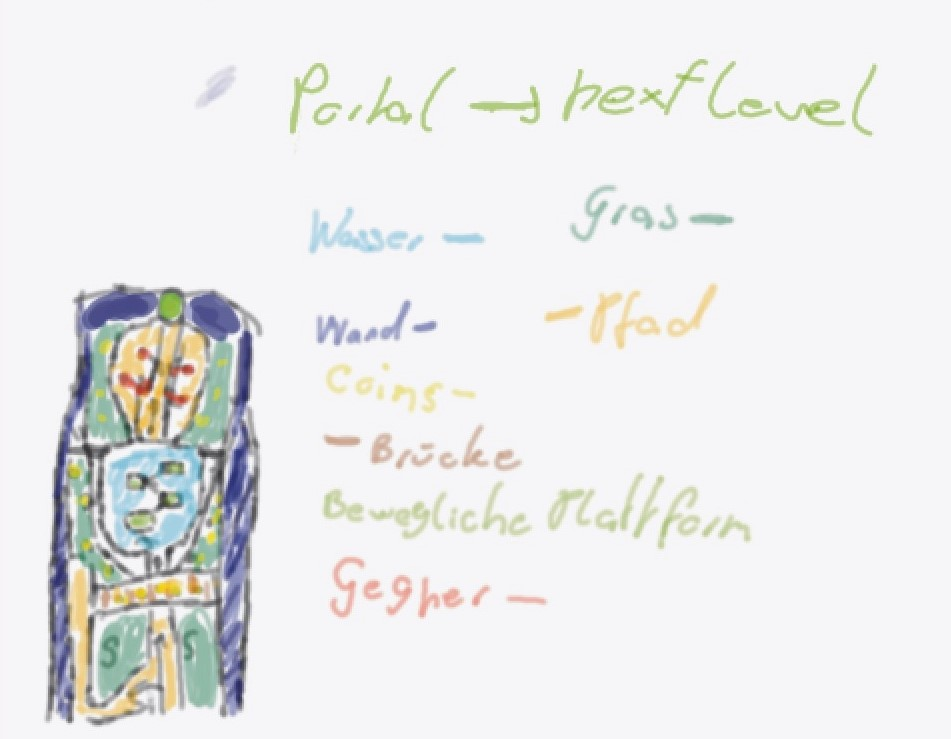
\includegraphics[width=\textwidth]{chapters/04/images/V1/drawing.jpg}
      \caption{Konzeptzeichnung und Ideenfindung}
      \label{fig:PE01}
    \end{minipage}
    \hfill
    \begin{minipage}[b]{0.45\textwidth}
      \centering
      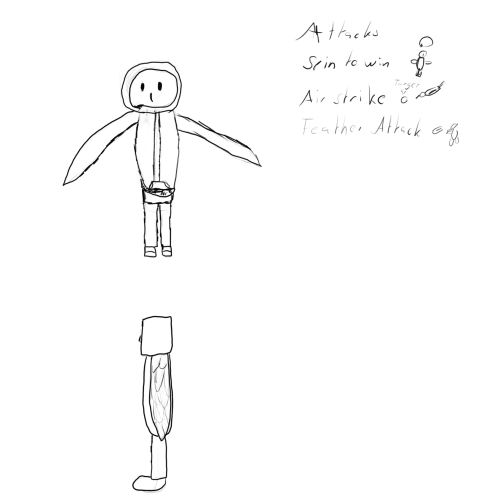
\includegraphics[width=\textwidth]{chapters/04/images/V1/CharScetch.png}
      \caption{Design des Hauptcharakters}
      \label{fig:PE02}
    \end{minipage}
    \caption{Idee und Anfangsschritte}
    \label{fig:IdeeThema}
  \end{figure}

  In der linken Abbildung sieht man die Konzeptzeichnung für das erste Level. In der Zeichnung ist eine von hohen Felsen abegrenzte Welt dargestellt. In der Mitte führt ein Pfad zu einem See. Über diesen schweben Plattformen. Vor dem See über den Weg ist eine Holzbrücke auf der sich Münzen befinden. Die roten Punkte auf der anderen Seite des Wassers sind Gegner und am Ende des Pfades ist ein Portal das zum Nächsten Level führt.
  In der rechten Abbildung ist das erste Design des Hauptcharakters dargestellt. Die überlegung war, eine Kaputzentragende Eule mit einem Menschenkörper zu mischen. Die Zeichnung zeigt den Charakter von Vorne und von der Seite. Der Text in der zweiten Abbildung ist eine Ideensammlung für die verschiedenen Attacken des Charakters. 
\pagebreak

\section{Version 1 des Prototypen}
In der Version 1 des Prototyps lag die Hauptkonztration in der schnellen Entwicklung eines Grundgerüsts des eigentlichen Prototypen. Dieser kann dann in den nächsten Versionen des Prototypen erweitert und verbessert werden. Ähnlich wie bei der agilen Projektentwicklung wurde die Entwicklung des Prototypen in verschiedene \glqq Sprints \grqq unterteilt. \\

Die zwei Hauptziele der Version 1 des Prototyen waren: 
\begin{itemize}
  \item Gestaltung des ersten Spiellevels im Rahmen des ersten Prototyps
  \item Programmierung von beweglichen Plattformen und Test von der Charaktersteuerung
\end{itemize}

\subsection{Prototyp V1 - Erstes Level:}

\begin{figure}[h]
  \centering
  \includegraphics*[width=0.6\textwidth]{chapters/04/images/V1/V1.png}
  \caption{Die erste Version des ersten Levels entwickelt in Unity.}
  \label{fig:PE03}
\end{figure}

Das erste Level des Prototypen wurde mittels dem Unity Terrain Tools gemacht. Mit diesem Tool können erhöhung aus einer Platte erstellt werden. Mit diesem Tool können auch Objekte wie Gräser und Bäume dynamisch auf den Grund des Levels plaziert werden. Das Untiy-Tool kann genauso die Platform bemalen. Dieses Tool ist zwar sehr mächtig, jedoch hat es auch seine Schwächen. Nach dem das Grundgerüst fertig war mussten noch Assets wie Bäume, Münzen und Gegner erstellt werden. Diese wurden in Blender Designed und erstellt. Diese wurden dann in Blener als FBX Datei Importiert. Wichtig war beim Importieren, dass Unity und Blender ein Unterschiedliches Koordinaten System verwendet. 


% todo Über die erste version des ersten levels weiterschreiben und bissly über die probleme
%\todo{to be continued}


\pagebreak

\subsection{Programmierung der beweglichen Plattformen:}

Für die programmierung der beweglichen Plattformen wurde ein leeres Unity Projekt angelegt. Dies bietet die Möglichkeit, ohne Auswirkungen auf den Prototypen zu Testen. Ein weiterer Vorteil ist, dass bei fatalen Fehlern einfach komplett neu begonnen werden kann. 

\begin{figure}[h]
  \centering
  \includegraphics*[width=0.6\textwidth]{chapters/04/images/V1/MovingPlatformV1.png}
  \caption{Die Entwicklung der Beweglichen Plattform in einem leeren Projekt}
  \label{fig:PE04}
\end{figure}

In der Abbildung 6.5 ist die Erstellung der beweglichen Plattformen dargestellt. Das weiße Rechteck ist die eigentliche Plattform auf der der Charakter stehen kann. Die grüne Box außerhalb ist ein \gls{boxcollider} \footnote[1]{Ein Box-Collider ist}. Dieser wurde für dieses Bild für bessere Erkennbarkeit hinausgestreckt. Die drei Punkte neben und über der Plattform sind die Wegpunkte für die Route der Plattform. Diese werden in dem \verb+WayPointFollower+ Script angesprochen. \\

Ein Problem, das bei dem Testen mit einer Spielfigur aufgetreten ist, war das die Plattform unter dem Charakter weggeflogen ist. Dabei hilft aber das \verb+StickyPlatform+ Script. In diesem wird mit einem genialen Trick dieses Problem gelöst.\\

Das \verb+WayPointFollower+ Script und auch das \verb+StickyPlatform+ Script werden in dem nächsten Kapiteln genauer beschrieben. 

\pagebreak

\subsubsection{WayPointFollower Skript}

\begin{lstlisting}[language=CSharp,caption={FixedUpdate der WayPointFollower Klasse.},label=code:mainmenu]
public class WaypointFollower : MonoBehaviour
{
  GameObject[] waypoints;
  int direction = 1; // 1 for forward, -1 for backward

  void FixedUpdate()
  {
      if (Vector3.Distance(transform.position, waypoints[currentWaypointIndex].transform.position) < .1f)
      {
          currentWaypointIndex += direction;

          if (currentWaypointIndex >= waypoints.Length || currentWaypointIndex < 0)
          {
              direction *= -1; // Reverse the direction when reaching the end or start
              currentWaypointIndex += direction * 2; // Move two steps in the opposite direction
          }
      }

      transform.position = Vector3.MoveTowards(transform.position, waypoints[currentWaypointIndex].transform.position, speed * Time.deltaTime);
  }
}
\end{lstlisting}

In dem oben abgebildeten Listing 6.1 ist ein Ausschnitt der \verb+WayPointFollower+ Klasse dargestellt. Die in Unity erstellten Wegpunkte werden in das GameObject Array gespeichert. Mittels dem Index\footnote[1]{Index ist eine Stelle in einem Array.} und der \verb+direction+ Variable wird durch dieses Array durchiteriert\footnote[2]{Iterieren ist der Prozess des durchlaufen einer Sammlung von Daten.}. Wenn der Index außerhalb des Arrays von Wegpunkten angekommen ist, dann wird die \verb+direction+ umgedreht. Für die eigentliche Bewegung der Plattform ist die Methode \verb+Vector3.MoveTowards+ verantwortlich. In dieser wird die aktuelle Position, die Position des Ziels und die sich zu bewegende Entfernung übergeben.


\pagebreak

\subsubsection{StickyPlatform Skript}

\begin{lstlisting}[language=CSharp,caption={StickyPlatform Klasse.},label=code:mainmenu]
  public class StickyPlatform : MonoBehaviour
  {
      public string playerTag = "Player";
  
      private void OnCollisionEnter(Collision collision)
      {
          // Check if the colliding object has the specified tag.
          if (collision.gameObject.CompareTag(playerTag))
          {
              // Reset the player's velocity to prevent unexpected behavior.
              Rigidbody playerRigidbody = collision.gameObject.GetComponent<Rigidbody>();
              if (playerRigidbody != null)
              {
                  playerRigidbody.velocity = Vector3.zero;
              }
  
              // Set the platform as the parent of the player's transform.
              collision.gameObject.transform.SetParent(transform);
          }
      }
  
      private void OnCollisionExit(Collision collision)
      {
          if (collision.gameObject.CompareTag(playerTag))
          {
              // When the player exits the collision, remove the parent relationship.
              collision.gameObject.transform.SetParent(null);
          }
      }
  }
\end{lstlisting}

In dem Listing 6.2 ist ein Ausschnitt des Codes von der StickyPlatform Klasse zu sehen. Der geniale Trick der in dieser Klasse verwendet wird ist, dass der \verb+Player+ zu einem \verb+Child+ von der beweglichen Plattform gemacht wird. Das bewirkt, dass die Plattform \glqq sticky\grqq ist. Also bewegt sich der Spieler, solange er sich auf dieser Plattform befindet, relativ zu der Plattform.

\pagebreak

\subsection{Herausforderungen und Fortschritt:}
\begin{itemize}
  \item Bewältigung technischer Herausforderungen während der V1-Entwicklung
  \item Erkennung von Leistungsproblemen aufgrund von Polygonanzahlen
  \item Vorbereitung für die Optimierung in Version 2 des Prototyps (V2)
\end{itemize}


\pagebreak

\section{Version 2 des Prototyps}

\begin{itemize}
  \item Optimierung und Fortschritt:
    \begin{itemize}
      \item Weiterentwicklung des Prototyps zu Version 2 (V2) zur Leistungsoptimierung und Verbesserung der Spielmechanik
      \item Design und Implementierung des Benutzeroberflächen-Designs (UI), einschließlich Hauptmenü, Pausemenü und Ingame-UI
      \item Erstellung zusätzlicher Spielassets wie Bäume, bewegliche Plattformen, Steine, Fässchen und Münzen
    \end{itemize}
\end{itemize}

Bei der Version 2 unseres Prototypen ist die Herausforderung gewesen die Assets performanteren Stand zu bringen. Der Grund dafür war das sich rausgestellt hatte das zwar die Assets zwar optisch gut waren aber die Perfomance lied deutlich darunter. Um das zu verhindern mussten alle Objekte nochmal überarbeitet werden sowie die Hauptfigur. Nach der Überarbeitung ist die Perfomance besser geworden.

\pagebreak

\section{Finaler Prototyp}

\begin{itemize}
  \item Abschlussarbeiten am Prototyp:
    \begin{itemize}
      \item Fertigstellung des ersten Levels im finalen Prototyp
      \item Konzeption und Aufbau des zweiten Spiellevels
      \item Umgestaltung und Optimierung des gesamten Benutzeroberflächen-Designs
    \end{itemize}
    
  \item Zusammenfassung und Ausblick:
    \begin{itemize}
      \item Zusammenführung der Entwicklungsphasen zu einem finalen Prototypen
      \item Fortlaufende Arbeit an der Fertigstellung des zweiten Levels und Feinschliff des Spielerlebnisses
      \item Ziel, ein ansprechendes und unterhaltsames Spielerlebnis zu bieten
    \end{itemize}
\end{itemize}



\pagebreak

